\section{Farmaci anti--ipertensivi}

\begin{tikzpicture}
	\Tree
	[.Anti-ipertensivi diuretici simpaticolitici vasodilatatori ]
\end{tikzpicture}

\begin{tikzpicture}
	\Tree
	[.{Diuretici\\ (capitolo ah hoc)}
		[.{Diuretici dell'ansa} \node[farmaco]{furosemide}; ]
		[.{Inibitori del simporto\\ $\text{Na}^+\text{-Cl}^-$} \node[farmaco]{tiazidici}; ]
		[. {Risparmiatori di $\text K^+$} \node[farmaco]{spironolattone}; ]
	]
\end{tikzpicture}

\begin{tikzpicture}
	\tikzset{level 3/.style={level distance=120pt}}
	\Tree
	[.Simpaticolitici
		[.{SNC}
			[.\node[farmaco]{$\alpha$-metildopa}; {Inibitore dopa-carbossilasi\\ emergenza ipertensiva \\ Da sedazione, tossicit\`a epatica\\ coombs positivo} ]
			[.\node[farmaco]{clonidina}; {Agonista $\alpha_2$. $\downarrow$noradrenalina\\ Usato in gravidanza \\ Da sonnolenza, depressione\\ $\downarrow$libido, secchezza fauci } ]
		]		
		[.{$\beta$--bloccanti}
			[.\node[farmaco]{propranololo}; {Usato in ipertensione, scompenso cardiaco, \\ aritmie, glaucoma. Produce $\downarrow$GC e renina. \\ Da affaticamento,$\downarrow$umore, insomnia, $\uparrow$glicemia, \\ alterazione assetto lipidico (i non ASI). \\ Interruzione improvvisa $\uparrow$infarto.} ]
		]		
		[.{$\alpha$--agonisti} \node[farmaco]{doxazosina}; ]
		[.{Misti $\alpha$/$\beta$}
			[.\node[farmaco]{labetalolo}; {ipertensione da feocromocitoma.\\ Da prurito intenso, $\downarrow$eiaculazione} ]
		]
	 ]
\end{tikzpicture}

\begin{tikzpicture}
	\tikzset{level distance=80pt, level 4/.style={level distance=100pt}}
	\Tree
	[.{Vasodilatatori}
		[.{diretti}
			[.{prevalentemente\\ arteriosi}
				[.{Inibitori IP3} \node[farmaco]{idralazina\\ (non pi\`u usato)}; ]
				[.{Ca${}^{2+}$ antagonisti}  \node[farmaco]{nifedipina\footnotemark\\ (anche verapamil\\ e diltiazem\\ ma su cuore)}; ]
			]
			[.{arterovenosi} 
				[.{rilascio NO} \node[farmaco]{nitroprussiato\footnotemark\\ nitroglicerina}; ]
			]
		]
		[.{indiretti}
			[.{ACE inibitori}
				[.\node[farmaco]{captopril\\ enalapril\\ fosinopril}; {Dilata arteriole e grandi vene. \\$\downarrow$pre/post carico. \\ Non inficia riflesso barocettivo\\ ne secrezione di aldosterone. \\ $\uparrow$bradichinina da tosse secca\\ e edema angioneurotico.} ]
			]
			[.{Antagonisti AT--1}
				[.{sartani} {Uso in ipertensione, ACC, \\ nefropatia diabetica\\ NO in gravidanza} ]
			]
		]
	]
\end{tikzpicture}

\footnotetext{Vedere farmaci angina}

\footnotetext{Vedere farmaci angina}

\newpage

\section{Farmaci nell'angina e infarto cardiaco}

\begin{tikzpicture}
	\Tree
	[.{angina\\ infarto} vasodilatatori simpaticomimetici ]
\end{tikzpicture}

\begin{tikzpicture}
	\tikzset{level distance=90pt, level 3/.style={level distance=130pt}}
	\Tree
	[.{Vasodilatatori}
		[.Nitrati
			[.\node[farmaco]{Isosorbide mononitrato}; {Duranta d'azione pi\`u lunga} ]
			[.\node[farmaco]{Nitroglicerina}; {Rilascio NO, $\uparrow$cGMP, relax muscolatura lis.\\ Via sublinguale, transdermica, rapido assorbimento\\ grazie alla solubilit\`a lipidica}  ]	
		]
		[.{Ca${}^{2+}$ antagonisti}
			[.\node[farmaco]{verapamil\\ (diidropiridine)}; {$\downarrow$conduzione NSA. $\downarrow$ RVP} ]
			[.\node[farmaco]{diltiazem}; {$\downarrow$conduzione NSA. $\downarrow$ RVP} ]
			[.\node[farmaco]{nifedipina}; {$\updownarrow$conduzione NSA.  Possibile tachicardia riflessa\\ minori effetti cardiaci} ]
		]
	]
\end{tikzpicture}

\begin{tikzpicture}
	\tikzset{level distance=90pt, level 3/.style={level distance=130pt}}
	\Tree
	[.{Simpaticolitici}
		[.{$\beta$--bloccanti}
			[.\node[farmaco]{propranololo\footnotemark}; {$\downarrow$GC, $\downarrow$PA, $\downarrow$consumo O${}_2$ micardico} ]
		]
	]
\end{tikzpicture}

\footnotetext{vedi farmaci anti-ipertensivi}

\begin{tikzpicture}
	\node[chartnode,anchor=west] at(0,0)(mlck){MLCK} node[chartnode,xshift=125pt] (mlckstar){MLCK${}^*$};
	\draw[drawarrow](mlck)[yshift=10pt]--node[smallfont,yshift=6pt,midway](Ca){Ca${}^{2+}$}
				node[chartnode,yshift=50pt,midway](CCa){Canali Ca${}^{2+}$}
				node[smallfont,yshift=-15pt,midway](camp){cAMP}
				node[chartnode,yshift=-60pt,midway](atp){ATP}(mlckstar);
	\draw[drawarrow] (mlckstar) [yshift=-10pt] -- (mlck);
	\draw[drawarrow] (CCa)-- node[midway](CCCa){} node[smallfont,xshift=5em](bloc){bloccanti canali} (Ca);
	\draw[drawarrow] (bloc)-- node[midway, below]{$\ominus$} (CCCa);
	\draw[drawarrow] (atp)-- node[midway](catp){} node[smallfont,xshift=5em](beta){$\beta$-bloccanti} (camp);
	\draw[drawarrow] (beta)-- node[midway, above]{$\oplus$} (catp);
	
	\node[chartnode,below right=1em and 2em of mlckstar](mlc){MLC};
	\node[chartnode,right=50pt of mlc](mlcstar){MLC${}^*$} node[right=3pt of mlcstar](+){+}
		node[chartnode, right=3pt of +](actina){actina};
	\node[chartnode,above=20pt of actina](contrazione){contrazione};
	\node[chartnode,below=20pt of mlc](relax){relax};
	\draw[drawarrow] (mlc) [yshift=10pt]-- node[midway](a){}(mlcstar);
	\draw[drawarrow] (mlcstar) [yshift=-10pt]-- 
		node[smallfont,midway,yshift=-6pt](cgmp){cGMP} 
		node[chartnode,yshift=-57pt,midway](gtp){GTP}
		(mlc);
	\draw[drawarrow] (actina) -- (contrazione);
	\draw[drawarrow] (mlc) -- (relax);
	\draw[drawarrow] (mlckstar) -| (a);
	\draw[drawarrow] (gtp)-- node[midway](cgtp){} 
		node[smallfont,xshift=10pt](gcstar){GC${}^*$}
		node[chartnode,xshift=100pt](gc){Guanil ciclasi} 
		(cgmp);
	\draw[drawarrow] (gc)-- node[midway](cgc){} node[midway, chartnode,yshift=-50pt](no){NO} (gcstar);
	\draw[drawarrow] (no)--node[midway, right]{$\oplus$}(cgc);
	
	\node[smallfont,text width=12em,anchor=west] at(0,-4) {* $\equiv$ elemento attivato\\
	MLCK $\equiv$ Miosina Catena Leggera chinasi\\ MLC $\equiv$ Miosina Catena Leggera};
\end{tikzpicture}

\begin{tikzpicture}
	\Tree
	[.Angina 
		[.{ischemia cardiaca transitoria\\ senza danno al miocardio}
			{stabile}
			{instabile}
			{di prinzmetal}
			{silente}
			{cronica}
		]
	]		
\end{tikzpicture}

\begin{tikzpicture}
	\Tree
	[.Terapia
		comportamentale
		chirurgica
		[.farmacologica
			[.{vasodilatatori\\ NO e Ca${}^2$ antagonisti}
				{per aumentare il flusso}
			]
			[.antiaggreganti {per evitare i trombi}
			]
			[.fibrinolitici {per distruggere i\\ trombi preesistenti}
			]
			[.{$\beta$ bloccanti} {per ridurre il fabbisogno energetico}
			]
			[.oppioidi {per ridurre il dolore}
			]
		]
	]
\end{tikzpicture}

\begin{tikzpicture}
	\Tree
	[.terapia
		[.stabile
			{nitrati organici}
			{$\beta$ bloccanti}
			{statina}
			{aspirina}
		]
		[.instabile
			{nitrati}
			{aspirina}
			{eparina}
		]
		[.variante
			{nitrati organici}
			{Ca${}^2$ antagonisti}
		]
	]	
\end{tikzpicture}

\textsc{Nitrati organici}

\begin{tikzpicture}
	\Tree
	[.{nitrati organici}
		{nitroglicerina}
		{isosorbide mononitrato}
	]
\end{tikzpicture}

\begin{tikzpicture}
	\Tree
	[.effetti
		[.{diminuzione della richiesta\\ di O${}_2$}
			{$\downarrow$ritorno venoso}
			{$\downarrow$volume intracardiaco}
			{$\downarrow$pressione arteriosa}
		]
		[.{scompasa spasmo arterioso} {vasodilatazione arterie\\ coronariche}
		]
	]
\end{tikzpicture}

\begin{tikzpicture}
	\Tree
	[.{effetti collaterali}
		{tachicardia riflessa}
		{aumento riflesso contrattile}
		{riduzione del tempo di perfusione\\ diastolica indotta da tachicardia}
	]
\end{tikzpicture}

\textsc{Calcio antagonisti}

\begin{tikzpicture}
	\Tree
	[.tipo
		[.L
			[.{Corrente lunga}
				[.Verapamil
					{cuore}
					{muscolo scheletrico\\ e liscio}
					{neuroni}
					{ossa}
				]
			]
		]
		[.T
			[.{Corrente breve}
				[.Flunarizina
					{cuore}
					{neuroni}
				]
			]
		]
		[.N
			[.{Corrente breve} {neuroni} 
			]
		]
		[.P
			[.{Corrente lunga} {neuroni} 
			]
		]
		[.{Q/R}
			[.{Segnapassi} {neuroni} 
			]
		]
	]
\end{tikzpicture}

\begin{tikzpicture}
	\Tree
	[.effetti
		[.{muscolo liscio}
		]
		[.{miocardio}
		]
		[.{muscolo scheletrico}
		]
	]
\end{tikzpicture}

\textsc{$\beta$-bloccati}

\newpage
